\section{Why Persistence Rises With Age: Skill at Entry and the Parents' Schooling}\label{sec:skill}

The IGE rises with age because what sons of richer parents bring to the labor market pays more as they age. In the
NLSY79, where the son's tested skill is measured before he enters the labor market, that skill carries three fifths of
the rise of the IGE between 25--29 and 50--54, and the parents' schooling beyond it most of the rest
(Table~\ref{tab:skill_entry}). In the PSID the rise happens within occupations and is predicted by the job a son holds
at 25--34 and by his schooling, whose return rises with age. Everything here is descriptive: skill, schooling and jobs
are outcomes of the same background.

\subsection{Skill at entry}

The NLSY79 follows sons born 1957--64 to their late fifties, and their earnings IGE rises from 0.340$^{***}$ at 25--29 to
0.506$^{***}$ at 50--54, an opening of 0.166$^{***}$ ($p<0.001$). The split of Section~\ref{sec:passedon}, applied to what
the 1979 interview records about the parents---the occupation and work of the adult man and woman at 14, region, the
parents' schooling and reading materials at home---assigns 0.120$^{***}$ ($p<0.001$) of the opening to the parents'
schooling and reading, and nothing to the parents' occupation wage (1.1\%, $p = 0.35$).\footnote{2,952 sons; 1979
weights; 200 cluster-bootstrap draws of 1979 households. Code: \texttt{86.NLSY79YouthWhatIsPassedOn.py}.} The father's
schooling carries the rising part: 0.016 at 25--29, 0.044$^{***}$ at 35--39 and 0.076$^{***}$ at 50--54, the same shape as
in the PSID (0.014 to 0.075$^{***}$ at 45--49; Section~\ref{sec:passedon}).

Adding the son's AFQT, measured in 1980 at ages 15--23, shows how much of that is the son's skill at entry. The AFQT
carries 28.0\%$^{***}$ of the IGE over 25--59, and its contribution rises from 0.077$^{***}$ at 25--29 to 0.181$^{***}$ at
50--54: an opening of 0.103$^{***}$ ($p<0.001$), 62 percent of the opening of the IGE. Seven tenths of the father's
schooling share runs through the son's AFQT (0.027$^{***}$ of 0.039$^{***}$), and two fifths of its rise with age
(0.025$^{***}$ of 0.060$^{***}$). The parents' schooling and reading beyond the AFQT still open by 0.059$^{***}$
($p = 0.004$), and the rest no longer opens (0.003, against 0.048 without the AFQT).\footnote{AFQT-3 (2006 revision),
standardised within birth year over the civilian sample with 1979 weights. Code: \texttt{87.NLSY79YouthAFQT.py}
(\texttt{output/nlsy79\_youth\_afqt.md}).} The AFQT is measured after some of the son's own schooling, so it is his
skill when he enters the labor market, not an endowment.

The rise is age, not the rise of the skill premium in the 1980s and 1990s. The NLSY79 sons reach their late twenties
in 1982--93 and their forties in 1997--2008, when the return to skill was rising nationally. The NLSY97 sons, born
1980--84, reach the same ages twenty years later. In their IGE the AFQT's contribution rises from 0.033$^{***}$ at
25--29 to 0.054$^{***}$ at 40--44 (an opening of 0.021$^{**}$, $p = 0.027$), a factor of 1.64; in the NLSY79 it rises
over the same ages from 0.077$^{***}$ to 0.131$^{***}$, a factor of 1.70 (panel B of Table~\ref{tab:age_period}). In the
hourly wage the NLSY97 contribution opens by 0.029$^{***}$, 43 percent of the opening of the wage IGE.\footnote{The NLSY97
measures parental income in one year, which attenuates the IGE and the AFQT's gradient in parental income alike; the
comparison is of the rise within each cohort. Code: \texttt{94.NLSY97AFQT.py}.}

\begin{table}[!htbp]
\centering
\caption{Why the IGE rises with age: the son's skill at entry and the parents' schooling (NLSY79)}
\label{tab:skill_entry}
\resizebox{\ifdim\width>\textwidth\textwidth\else\width\fi}{!}{%
\resizebox*{!}{\ifdim\totalheight>0.85\textheight 0.85\textheight\else\totalheight\fi}{%
\begin{tabular}{lcccccc}
\toprule
 & \begin{tabular}[b]{@{}c@{}}25--29\end{tabular} & \begin{tabular}[b]{@{}c@{}}35--39\end{tabular} & \begin{tabular}[b]{@{}c@{}}45--49\end{tabular} & \begin{tabular}[b]{@{}c@{}}50--54\end{tabular} & \begin{tabular}[b]{@{}c@{}}25--59\end{tabular} & \begin{tabular}[b]{@{}c@{}}Opening\\50--54 minus\\25--29\end{tabular} \\
 & (1) & (2) & (3) & (4) & (5) & (6) \\
\midrule
\multicolumn{7}{l}{\textit{A. Sons, pooled}} \\
IGE & $0.340^{***}$ & $0.413^{***}$ & $0.486^{***}$ & $0.506^{***}$ & $0.407^{***}$ & $0.166^{***}$ \\
 & (0.022) & (0.027) & (0.035) & (0.042) & (0.022) & (0.037) \\
The son's AFQT & $0.077^{***}$ & $0.123^{***}$ & $0.157^{***}$ & $0.181^{***}$ & $0.114^{***}$ & $0.103^{***}$ \\
 & (0.010) & (0.013) & (0.016) & (0.020) & (0.011) & (0.017) \\
Father's schooling, without the son's AFQT & $0.016$ & $0.044^{***}$ & $0.066^{***}$ & $0.076^{***}$ & $0.039^{***}$ & $0.060^{***}$ \\
 & (0.012) & (0.015) & (0.021) & (0.022) & (0.011) & (0.022) \\
Father's schooling, with the son's AFQT & $-0.002$ & $0.014$ & $0.026$ & $0.033$ & $0.012$ & $0.035^{*}$ \\
 & (0.012) & (0.014) & (0.019) & (0.021) & (0.011) & (0.020) \\
Parents' schooling and reading, without AFQT & $0.050^{***}$ & $0.115^{***}$ & $0.151^{***}$ & $0.170^{***}$ & $0.102^{***}$ & $0.120^{***}$ \\
 & (0.013) & (0.017) & (0.019) & (0.022) & (0.013) & (0.021) \\
Parents' schooling and reading, with AFQT & $0.005$ & $0.037^{**}$ & $0.054^{***}$ & $0.064^{***}$ & $0.033^{**}$ & $0.059^{***}$ \\
 & (0.014) & (0.017) & (0.018) & (0.020) & (0.013) & (0.021) \\
Rest, without AFQT & $0.277^{***}$ & $0.273^{***}$ & $0.295^{***}$ & $0.325^{***}$ & $0.280^{***}$ & $0.048$ \\
 & (0.029) & (0.035) & (0.041) & (0.049) & (0.028) & (0.044) \\
Rest, with AFQT & $0.255^{***}$ & $0.241^{***}$ & $0.243^{***}$ & $0.258^{***}$ & $0.245^{***}$ & $0.003$ \\
 & (0.028) & (0.035) & (0.039) & (0.048) & (0.027) & (0.043) \\
Father's schooling through the son's AFQT & $0.018^{***}$ & $0.029^{***}$ & $0.040^{***}$ & $0.043^{***}$ & $0.027^{***}$ & $0.025^{***}$ \\
 & (0.003) & (0.005) & (0.007) & (0.008) & (0.004) & (0.007) \\
\addlinespace
\multicolumn{7}{l}{\textit{B. White sons}} \\
IGE & $0.292^{***}$ & $0.407^{***}$ & $0.445^{***}$ & $0.480^{***}$ & $0.373^{***}$ & $0.188^{***}$ \\
 & (0.028) & (0.037) & (0.046) & (0.055) & (0.029) & (0.048) \\
The son's AFQT & $0.052^{***}$ & $0.092^{***}$ & $0.115^{***}$ & $0.143^{***}$ & $0.082^{***}$ & $0.091^{***}$ \\
 & (0.010) & (0.014) & (0.018) & (0.022) & (0.012) & (0.018) \\
Father's schooling, without the son's AFQT & $0.015$ & $0.055^{***}$ & $0.080^{***}$ & $0.083^{***}$ & $0.044^{***}$ & $0.067^{**}$ \\
 & (0.015) & (0.019) & (0.027) & (0.029) & (0.015) & (0.028) \\
Father's schooling, with the son's AFQT & $-0.002$ & $0.023$ & $0.035$ & $0.035$ & $0.015$ & $0.038$ \\
 & (0.015) & (0.018) & (0.024) & (0.026) & (0.014) & (0.026) \\
Parents' schooling and reading, without AFQT & $0.035^{**}$ & $0.112^{***}$ & $0.150^{***}$ & $0.172^{***}$ & $0.096^{***}$ & $0.137^{***}$ \\
 & (0.015) & (0.020) & (0.022) & (0.027) & (0.015) & (0.026) \\
Parents' schooling and reading, with AFQT & $-0.003$ & $0.038^{*}$ & $0.052^{**}$ & $0.065^{***}$ & $0.031^{**}$ & $0.068^{***}$ \\
 & (0.016) & (0.020) & (0.022) & (0.024) & (0.015) & (0.024) \\
Rest, without AFQT & $0.247^{***}$ & $0.281^{***}$ & $0.274^{***}$ & $0.311^{***}$ & $0.261^{***}$ & $0.064$ \\
 & (0.035) & (0.044) & (0.050) & (0.060) & (0.034) & (0.053) \\
Rest, with AFQT & $0.239^{***}$ & $0.269^{***}$ & $0.251^{***}$ & $0.273^{***}$ & $0.247^{***}$ & $0.034$ \\
 & (0.034) & (0.042) & (0.047) & (0.058) & (0.033) & (0.053) \\
Father's schooling through the son's AFQT & $0.018^{***}$ & $0.032^{***}$ & $0.045^{***}$ & $0.047^{***}$ & $0.029^{***}$ & $0.030^{***}$ \\
 & (0.004) & (0.006) & (0.009) & (0.010) & (0.005) & (0.009) \\
\bottomrule
\end{tabular}}}
\par\smallskip
\begin{minipage}{\textwidth}\footnotesize \textit{Continued on the next table; notes below its last part.}\end{minipage}
\end{table}
\begin{table}[!htbp]
\centering
\addtocounter{table}{-1}
\caption{Why the IGE rises with age: the son's skill at entry and the parents' schooling (NLSY79) (continued)}
\resizebox{\ifdim\width>\textwidth\textwidth\else\width\fi}{!}{%
\resizebox*{!}{\ifdim\totalheight>0.85\textheight 0.85\textheight\else\totalheight\fi}{%
\begin{tabular}{lcccccc}
\toprule
 & \begin{tabular}[b]{@{}c@{}}25--29\end{tabular} & \begin{tabular}[b]{@{}c@{}}35--39\end{tabular} & \begin{tabular}[b]{@{}c@{}}45--49\end{tabular} & \begin{tabular}[b]{@{}c@{}}50--54\end{tabular} & \begin{tabular}[b]{@{}c@{}}25--59\end{tabular} & \begin{tabular}[b]{@{}c@{}}Opening\\50--54 minus\\25--29\end{tabular} \\
 & (1) & (2) & (3) & (4) & (5) & (6) \\
\midrule
\multicolumn{7}{l}{\textit{C. Black sons}} \\
IGE & $0.298^{***}$ & $0.233^{***}$ & $0.365^{***}$ & $0.362^{***}$ & $0.305^{***}$ & $0.064$ \\
 & (0.034) & (0.040) & (0.058) & (0.056) & (0.031) & (0.060) \\
The son's AFQT & $0.067^{***}$ & $0.087^{***}$ & $0.088^{***}$ & $0.106^{***}$ & $0.080^{***}$ & $0.039^{*}$ \\
 & (0.016) & (0.019) & (0.024) & (0.026) & (0.017) & (0.021) \\
Father's schooling, without the son's AFQT & $0.003$ & $-0.006$ & $0.000$ & $0.027^{*}$ & $0.003$ & $0.023$ \\
 & (0.007) & (0.010) & (0.013) & (0.015) & (0.006) & (0.015) \\
Father's schooling, with the son's AFQT & $-0.002$ & $-0.014$ & $-0.009$ & $0.016$ & $-0.003$ & $0.018$ \\
 & (0.007) & (0.010) & (0.013) & (0.013) & (0.006) & (0.015) \\
Parents' schooling and reading, without AFQT & $0.052^{***}$ & $0.085^{***}$ & $0.118^{***}$ & $0.104^{***}$ & $0.074^{***}$ & $0.052^{*}$ \\
 & (0.017) & (0.021) & (0.030) & (0.033) & (0.017) & (0.030) \\
Parents' schooling and reading, with AFQT & $0.017$ & $0.032$ & $0.065^{**}$ & $0.047$ & $0.030^{*}$ & $0.031$ \\
 & (0.018) & (0.020) & (0.029) & (0.031) & (0.016) & (0.030) \\
Rest, without AFQT & $0.274^{***}$ & $0.131^{***}$ & $0.210^{***}$ & $0.229^{***}$ & $0.225^{***}$ & $-0.044$ \\
 & (0.046) & (0.045) & (0.066) & (0.065) & (0.038) & (0.071) \\
Rest, with AFQT & $0.250^{***}$ & $0.099^{**}$ & $0.184^{***}$ & $0.186^{***}$ & $0.195^{***}$ & $-0.064$ \\
 & (0.045) & (0.046) & (0.066) & (0.063) & (0.036) & (0.070) \\
Father's schooling through the son's AFQT & $0.005^{**}$ & $0.008^{**}$ & $0.009^{**}$ & $0.010^{**}$ & $0.006^{**}$ & $0.005$ \\
 & (0.002) & (0.004) & (0.004) & (0.005) & (0.003) & (0.004) \\
\bottomrule
\end{tabular}}}
\par\smallskip
\begin{minipage}{\textwidth}\footnotesize \textit{Notes:} Contributions to the IGE of sons' ln annual earnings on ln parental income (mean 1978--80) in each age band; exact Gelbach split with the components of Table~\ref{tab:passed_on_data}, column (4), without (A) and with (B) the son's AFQT (AFQT-3, 1980 ASVAB at ages 15--23, standardised within birth year). 'Through the son's AFQT' = the father's-schooling contribution without minus with AFQT, on common bootstrap draws. NLSY79 Black and White youths living with a parent in 1979--81; 1979 weights; 200 cluster-bootstrap draws of 1979 households. Source: \texttt{IGE/86.NLSY79YouthWhatIsPassedOn.py}, \texttt{IGE/87.NLSY79YouthAFQT.py}; table built by \texttt{IGE/90.PaperBRaceNeutralTables.py}. $^{***}$ $p<0.01$, $^{**}$ $p<0.05$, $^{*}$ $p<0.1$.\end{minipage}
\end{table}


The age pattern says why skill at entry pays more later. Under employer learning the return to what employers see at
hiring, schooling, falls with experience while the return to what they learn, ability, rises
\citep{altonji2001employer, lange2007speed}. In the NLSY79 both rise: with the AFQT and schooling in the same
regression, the return to schooling rises by 0.049$^{***}$ from the bands below 35 to the bands above, and the return to
the AFQT by 0.036$^{***}$ (Appendix Table~\ref{tab:afqtgrowth}). Skill and schooling acquired before entry are
complements of the human capital accumulated on the job \citep{bhuller2017life}, and the sons who bring more of them
accumulate faster.

\subsection{Where in the career}

The rise is within occupations. Each son's log wage is split into the CPS wage score of his occupation and his wage
relative to it: the parental-income gradient of the log wage rises from 0.259$^{***}$ at 25--34 to 0.410$^{***}$ at
35--55, and the occupation part barely moves (0.158 to 0.176) while the within-occupation part more than doubles (0.102
to 0.235) (Figure~\ref{fig:career}, Table~\ref{tab:careerdecomp}).\footnote{All PSID occupation codes mapped to the
occ1990dd scheme; the score is the mean log hourly wage of men aged 25--64 in the occupation relative to all men, from
2.9 million CPS Outgoing Rotation Group records of 1979--2019. Code: \texttt{27.CareerWageGrowth.py}.} Background
buys a better-paid occupation at the start, and that advantage hardly grows; what grows is the wage within it.

\begin{figure}[!htbp]
\centering
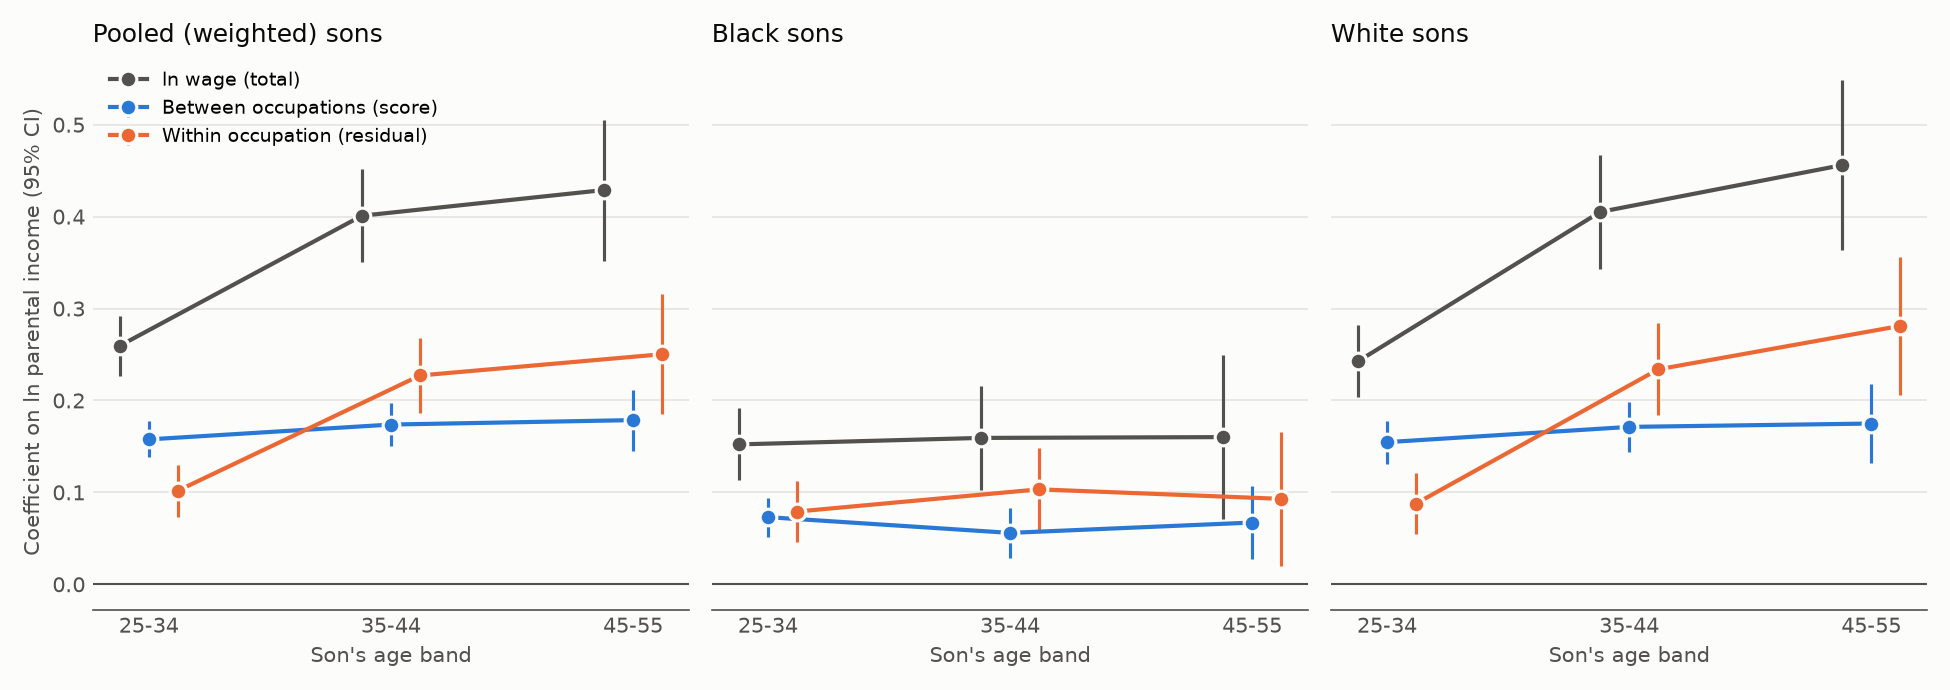
\includegraphics[width=\textwidth]{career_wage_growth.png}
\caption{Wage persistence by the son's age: between and within occupations (PSID)}\label{fig:career}
\begin{minipage}{\textwidth}\footnotesize \textit{Notes:} Coefficient of the son's log wage, of his occupation's wage
score and of his within-occupation residual on log parental income, by age band, with 95\% confidence intervals. The
score and the residual add up to the log wage. Code: \texttt{27.CareerWageGrowth.py}.\end{minipage}
\end{figure}

\begin{table}[!htbp]
\centering
\caption{Wage persistence by age: between and within occupations (PSID, sons)}
\label{tab:careerdecomp}
\resizebox{\ifdim\width>\textwidth\textwidth\else\width\fi}{!}{%
\resizebox*{!}{\ifdim\totalheight>0.85\textheight 0.85\textheight\else\totalheight\fi}{%
\begin{tabular}{lcccc}
\toprule
Panel / row & \begin{tabular}[b]{@{}c@{}}ln wage\end{tabular} & \begin{tabular}[b]{@{}c@{}}Occupation\\score\end{tabular} & \begin{tabular}[b]{@{}c@{}}Within-\\occupation\\residual\end{tabular} & \begin{tabular}[b]{@{}c@{}}Share\\between\\(2)/(1)\end{tabular} \\
 & (1) & (2) & (3) & (4) \\
\midrule
\multicolumn{5}{l}{\textit{Pooled (weighted): coefficient on log parental income}} \\
Sons aged 25--34 & $0.259^{***}$ & $0.158^{***}$ & $0.102^{***}$ & $0.608^{***}$ \\
 & (0.017) & (0.010) & (0.014) & (0.038) \\
Sons aged 35--44 & $0.401^{***}$ & $0.174^{***}$ & $0.227^{***}$ & $0.433^{***}$ \\
 & (0.026) & (0.012) & (0.021) & (0.027) \\
Sons aged 45--55 & $0.429^{***}$ & $0.179^{***}$ & $0.250^{***}$ & $0.416^{***}$ \\
 & (0.039) & (0.017) & (0.033) & (0.037) \\
Sons aged 35--55 & $0.410^{***}$ & $0.176^{***}$ & $0.235^{***}$ & $0.428^{***}$ \\
 & (0.028) & (0.013) & (0.022) & (0.026) \\
Son-years (25--34 / 35--44 / 45--55) & 21,315 / 12,648 / 5,728 &  &  &  \\
\addlinespace
\multicolumn{5}{l}{\textit{Black: coefficient on log parental income}} \\
Sons aged 25--34 & $0.152^{***}$ & $0.073^{***}$ & $0.079^{***}$ & $0.480^{***}$ \\
 & (0.020) & (0.011) & (0.017) & (0.064) \\
Sons aged 35--44 & $0.159^{***}$ & $0.056^{***}$ & $0.103^{***}$ & $0.351^{***}$ \\
 & (0.029) & (0.014) & (0.023) & (0.069) \\
Sons aged 45--55 & $0.160^{***}$ & $0.067^{***}$ & $0.093^{**}$ & $0.420^{***}$ \\
 & (0.046) & (0.020) & (0.037) & (0.111) \\
Sons aged 35--55 & $0.161^{***}$ & $0.060^{***}$ & $0.101^{***}$ & $0.371^{***}$ \\
 & (0.030) & (0.014) & (0.024) & (0.068) \\
Son-years (25--34 / 35--44 / 45--55) & 7,412 / 4,149 / 1,843 &  &  &  \\
\addlinespace
\multicolumn{5}{l}{\textit{White: coefficient on log parental income}} \\
Sons aged 25--34 & $0.243^{***}$ & $0.155^{***}$ & $0.088^{***}$ & $0.638^{***}$ \\
 & (0.020) & (0.012) & (0.017) & (0.049) \\
Sons aged 35--44 & $0.405^{***}$ & $0.171^{***}$ & $0.234^{***}$ & $0.423^{***}$ \\
 & (0.032) & (0.014) & (0.026) & (0.030) \\
Sons aged 45--55 & $0.456^{***}$ & $0.175^{***}$ & $0.281^{***}$ & $0.383^{***}$ \\
 & (0.047) & (0.022) & (0.038) & (0.039) \\
Sons aged 35--55 & $0.418^{***}$ & $0.172^{***}$ & $0.246^{***}$ & $0.411^{***}$ \\
 & (0.033) & (0.015) & (0.026) & (0.028) \\
Son-years (25--34 / 35--44 / 45--55) & 13,915 / 8,500 / 3,885 &  &  &  \\
\addlinespace
\multicolumn{5}{l}{\textit{White $-$ Black: coefficient on log parental income}} \\
Sons aged 25--34 & $0.090^{***}$ & $0.082^{***}$ & $0.009$ & $0.903^{***}$ \\
 & (0.028) & (0.016) & (0.024) & (0.238) \\
Sons aged 35--44 & $0.246^{***}$ & $0.115^{***}$ & $0.131^{***}$ & $0.469^{***}$ \\
 & (0.043) & (0.020) & (0.035) & (0.071) \\
Sons aged 45--55 & $0.296^{***}$ & $0.108^{***}$ & $0.188^{***}$ & $0.364^{***}$ \\
 & (0.066) & (0.030) & (0.053) & (0.083) \\
Sons aged 35--55 & $0.258^{***}$ & $0.112^{***}$ & $0.145^{***}$ & $0.436^{***}$ \\
 & (0.045) & (0.020) & (0.035) & (0.065) \\
\bottomrule
\end{tabular}}}
\par\smallskip
\begin{minipage}{\textwidth}\footnotesize \textit{Continued on the next table; notes below its last part.}\end{minipage}
\end{table}
\begin{table}[!htbp]
\centering
\addtocounter{table}{-1}
\caption{Wage persistence by age: between and within occupations (PSID, sons) (continued)}
\resizebox{\ifdim\width>\textwidth\textwidth\else\width\fi}{!}{%
\resizebox*{!}{\ifdim\totalheight>0.85\textheight 0.85\textheight\else\totalheight\fi}{%
\begin{tabular}{lcccc}
\toprule
Panel / row & \begin{tabular}[b]{@{}c@{}}ln wage\end{tabular} & \begin{tabular}[b]{@{}c@{}}Occupation\\score\end{tabular} & \begin{tabular}[b]{@{}c@{}}Within-\\occupation\\residual\end{tabular} & \begin{tabular}[b]{@{}c@{}}Share\\between\\(2)/(1)\end{tabular} \\
 & (1) & (2) & (3) & (4) \\
\midrule
\multicolumn{5}{l}{\textit{Change in the coefficient across age bands (career divergence)}} \\
Pooled (weighted): (35--55) $-$ (25--34) & $0.151^{***}$ & $0.018^{*}$ & $0.133^{***}$ & $0.119^{*}$ \\
 & (0.023) & (0.010) & (0.021) & (0.062) \\
Pooled (weighted): (45--55) $-$ (25--34) & $0.169^{***}$ & $0.021$ & $0.148^{***}$ & $0.124$ \\
 & (0.035) & (0.015) & (0.032) & (0.081) \\
Black: (35--55) $-$ (25--34) & $0.009$ & $-0.013$ & $0.022$ &  \\
 & (0.025) & (0.011) & (0.022) &  \\
Black: (45--55) $-$ (25--34) & $0.008$ & $-0.006$ & $0.014$ &  \\
 & (0.042) & (0.019) & (0.036) &  \\
White: (35--55) $-$ (25--34) & $0.176^{***}$ & $0.017$ & $0.158^{***}$ & $0.099$ \\
 & (0.027) & (0.012) & (0.024) & (0.063) \\
White: (45--55) $-$ (25--34) & $0.213^{***}$ & $0.020$ & $0.193^{***}$ & $0.095$ \\
 & (0.042) & (0.020) & (0.037) & (0.084) \\
White $-$ Black: (35--55) $-$ (25--34) & $0.167^{***}$ & $0.031^{*}$ & $0.136^{***}$ & $0.184^{**}$ \\
 & (0.037) & (0.016) & (0.032) & (0.087) \\
White $-$ Black: (45--55) $-$ (25--34) & $0.206^{***}$ & $0.026$ & $0.179^{***}$ & $0.127$ \\
 & (0.060) & (0.027) & (0.051) & (0.117) \\
\bottomrule
\end{tabular}}}
\par\smallskip
\begin{minipage}{\textwidth}\footnotesize \textit{Notes:} One regression per cell: the son's outcome (column header) on log parental income (mean at 13--19), son-years in the age band, controls for quartics in the father's age at 16 and the son's age. Occupational wage score: mean log hourly wage of men aged 25--64 in the occupation relative to all men (CPS MORG, base 1992--2002), occupations harmonised to Dorn's occ1990dd scheme; log wage = score (between occupations) + residual (within occupation), so the score and residual columns add up to the log-wage column on the same sample. With a time-varying score (the same relative premium in $t-1$ to $t+1$) the between share of the change of the racial gap is 0.27 (\texttt{output/career\_wage\_growth.md}). Column (4) is left blank when the denominator is not different from zero. All cells are estimated as one stacked system, so differences across bands and groups have standard errors (clustered by 1968 family). Pooled: Black and White sons, weighted; Black and White: unweighted. Sons select into occupations, so the split is accounting, not causal. $^{***}$ $p<0.01$, $^{**}$ $p<0.05$, $^{*}$ $p<0.1$. Source: \texttt{27.CareerWageGrowth.py} (\texttt{output/career\_wage\_growth.csv}); table built by \texttt{28.PaperBTables.py}.\end{minipage}
\end{table}


The job a son holds at 25--34 predicts it. With fixed effects for his modal occupation-by-industry cell at 25--34,
whatever he does later, the parental-income coefficient at 35--55 falls by 0.405$^{***}$ of its rise after 35; his
detailed occupation alone accounts for 0.591$^{***}$ (Table~\ref{tab:earlyjob}).\footnote{93 percent of sons observed
at 35--55 have an early job; randomly reassigning cells gives shares of about 0.03. Code:
\texttt{35.EarlyIndustryLatePayoff.py}.} Access to the jobs whose wages keep growing is unequal by background: 20.2
percent of sons from the top third of parental incomes start in one, 4.7 percent from the bottom third
(Table~\ref{tab:access}). The early job also reflects the son's own skill, so these shares say how far where a son stands
at 25--34 predicts how far he pulls away, not what the job itself does.

\begin{table}[!htbp]
\centering
\caption{Where sons start: the job at 25--34 and the rise of wage persistence after 35 (PSID, sons)}
\label{tab:earlyjob}
\resizebox{\ifdim\width>\textwidth\textwidth\else\width\fi}{!}{%
\resizebox*{!}{\ifdim\totalheight>0.85\textheight 0.85\textheight\else\totalheight\fi}{%
\begin{tabular}{lcccccc}
\toprule
 & \begin{tabular}[b]{@{}c@{}}Accounted\\for at\\25--34\end{tabular} & \begin{tabular}[b]{@{}c@{}}Accounted\\for at\\35--55\end{tabular} & \begin{tabular}[b]{@{}c@{}}Change\end{tabular} & \begin{tabular}[b]{@{}c@{}}Share of\\pooled rise\end{tabular} & \begin{tabular}[b]{@{}c@{}}Change,\\White $-$ Black\end{tabular} & \begin{tabular}[b]{@{}c@{}}Share of\\gap change\end{tabular} \\
 & (1) & (2) & (3) & (4) & (5) & (6) \\
\midrule
\multicolumn{7}{l}{\textit{Fixed effects for the son's job at 25--34, by age band}} \\
Finance, insurance, legal, professional (example; 2 groups) & $0.014^{***}$ & $0.027^{***}$ & $0.013^{**}$ & $0.097^{**}$ & $0.012^{*}$ & $0.085^{*}$ \\
 & (0.003) & (0.007) & (0.005) & (0.039) & (0.006) & (0.046) \\
Industry groups ranked by pay and later growth (4 sets) & $0.024^{***}$ & $0.029^{***}$ & $0.005$ & $0.034$ & $0.001$ & $0.006$ \\
 & (0.005) & (0.008) & (0.005) & (0.037) & (0.008) & (0.058) \\
Industry group (33) & $0.034^{***}$ & $0.052^{***}$ & $0.018^{*}$ & $0.135^{*}$ & $0.015$ & $0.108$ \\
 & (0.007) & (0.013) & (0.010) & (0.072) & (0.016) & (0.105) \\
Manager or professional (2 groups) & $0.042^{***}$ & $0.076^{***}$ & $0.035^{***}$ & $0.257^{***}$ & $0.035^{***}$ & $0.246^{***}$ \\
 & (0.005) & (0.010) & (0.008) & (0.064) & (0.010) & (0.086) \\
Occupation group (11) & $0.057^{***}$ & $0.108^{***}$ & $0.051^{***}$ & $0.377^{***}$ & $0.045^{***}$ & $0.318^{***}$ \\
 & (0.007) & (0.013) & (0.010) & (0.078) & (0.015) & (0.111) \\
Occupation group + industry group (11 + 33) & $0.078^{***}$ & $0.129^{***}$ & $0.050^{***}$ & $0.376^{***}$ & $0.050^{**}$ & $0.352^{***}$ \\
 & (0.010) & (0.017) & (0.012) & (0.087) & (0.020) & (0.129) \\
Cells ranked by pay and later growth (4 sets) & $0.056^{***}$ & $0.093^{***}$ & $0.036^{***}$ & $0.271^{***}$ & $0.033^{***}$ & $0.237^{***}$ \\
 & (0.006) & (0.012) & (0.009) & (0.067) & (0.011) & (0.087) \\
Occupation $\times$ industry cell (11 $\times$ 33) & $0.091^{***}$ & $0.146^{***}$ & $0.054^{***}$ & $0.405^{***}$ & $0.070^{***}$ & $0.493^{***}$ \\
 & (0.011) & (0.020) & (0.015) & (0.099) & (0.025) & (0.171) \\
Detailed occupation (occ1990dd) & $0.086^{***}$ & $0.165^{***}$ & $0.079^{***}$ & $0.591^{***}$ & $0.101^{***}$ & $0.713^{***}$ \\
 & (0.011) & (0.020) & (0.017) & (0.120) & (0.026) & (0.211) \\
\bottomrule
\end{tabular}}}
\par\smallskip
\begin{minipage}{\textwidth}\footnotesize \textit{Notes:} Short regression: the son's log wage on log parental income in each age band (25--34, 35--55), controls as in Table~\ref{tab:industrydecomp}. Long regression: adds fixed effects for the son's job at 25--34 (row), estimated separately in each age band and race sample, so they absorb any wage profile of where he started, linear or not. Accounted for = short $-$ long. On this sample the pooled coefficient rises by 0.132$^{***}$ and the White $-$ Black gap changes by 0.140$^{***}$ from 25--34 to 35--55. Ranked sets: cells (or industries) in the top quartile of men's employment by CPS wage level and by CPS wage growth after 35, and their intersection. Permuting the cell labels across sons gives shares of about 0.03. The son's early job also reflects his own skills, so the rows measure how much where a son stands at 25--34 predicts how far he pulls away, not a causal payoff. 93\% of sons observed at 35--55 have a job at 25--34. Standard errors clustered by 1968 family. $^{***}$ $p<0.01$, $^{**}$ $p<0.05$, $^{*}$ $p<0.1$. Source: \texttt{35.EarlyIndustryLatePayoff.py} (\texttt{output/early\_industry\_late\_payoff.csv}); table built by \texttt{28.PaperBTables.py}.\end{minipage}
\end{table}

\begin{table}[!htbp]
\centering
\caption{Access to well-paid, fast-growing starting jobs at 25--34 (PSID, sons)}
\label{tab:access}
\resizebox{\ifdim\width>\textwidth\textwidth\else\width\fi}{!}{%
\resizebox*{!}{\ifdim\totalheight>0.85\textheight 0.85\textheight\else\totalheight\fi}{%
\begin{tabular}{lccccc}
\toprule
 & \begin{tabular}[b]{@{}c@{}}Well-paid,\\high later\\growth\\(a)\end{tabular} & \begin{tabular}[b]{@{}c@{}}Well-paid,\\high later\\growth\\(b)\end{tabular} & \begin{tabular}[b]{@{}c@{}}Well-paid,\\high later\\growth\\(c)\end{tabular} & \begin{tabular}[b]{@{}c@{}}Well-paid,\\high later\\growth\\(d)\end{tabular} & \begin{tabular}[b]{@{}c@{}}Well-paid,\\high later\\growth\\(e)\end{tabular} \\
 & (1) & (2) & (3) & (4) & (5) \\
\midrule
\multicolumn{6}{l}{\textit{Black and White sons (reference for terciles: Black, bottom tercile)}} \\
ln parental income & $0.104^{***}$ &  & $0.095^{***}$ &  & $0.002$ \\
 & (0.010) &  & (0.011) &  & (0.016) \\
White &  & $0.109^{***}$ & $0.042^{***}$ &  & $0.035^{*}$ \\
 &  & (0.014) & (0.016) &  & (0.020) \\
Black, middle tercile &  &  &  & $0.024$ &  \\
 &  &  &  & (0.022) &  \\
Black, top tercile &  &  &  & $0.125^{***}$ &  \\
 &  &  &  & (0.044) &  \\
White, bottom tercile &  &  &  & $0.048^{**}$ &  \\
 &  &  &  & (0.020) &  \\
White, middle tercile &  &  &  & $0.092^{***}$ &  \\
 &  &  &  & (0.017) &  \\
White, top tercile &  &  &  & $0.187^{***}$ &  \\
 &  &  &  & (0.017) &  \\
Rich White $-$ rich Black (top terciles) &  &  &  & $0.062$ &  \\
 &  &  &  & (0.045) &  \\
Father held a well-paid, high-later-growth job &  &  &  &  & $0.064^{**}$ \\
 &  &  &  &  & (0.025) \\
Years of education &  &  &  &  & $0.063^{***}$ \\
 &  &  &  &  & (0.005) \\
\addlinespace
\multicolumn{6}{l}{\textit{Black sons}} \\
ln parental income & $0.048^{***}$ &  & $0.048^{***}$ &  & $0.021$ \\
 & (0.009) &  & (0.009) &  & (0.018) \\
Middle tercile &  &  &  & $0.022^{*}$ &  \\
 &  &  &  & (0.013) &  \\
Top tercile &  &  &  & $0.104^{***}$ &  \\
 &  &  &  & (0.025) &  \\
Father held a well-paid, high-later-growth job &  &  &  &  & $0.008$ \\
 &  &  &  &  & (0.051) \\
Years of education &  &  &  &  & $0.052^{***}$ \\
 &  &  &  &  & (0.007) \\
\addlinespace
\multicolumn{6}{l}{\textit{White sons}} \\
ln parental income & $0.103^{***}$ &  & $0.103^{***}$ &  & $-0.001$ \\
 & (0.012) &  & (0.012) &  & (0.016) \\
Middle tercile &  &  &  & $0.050^{***}$ &  \\
 &  &  &  & (0.018) &  \\
Top tercile &  &  &  & $0.138^{***}$ &  \\
 &  &  &  & (0.019) &  \\
Father held a well-paid, high-later-growth job &  &  &  &  & $0.048^{**}$ \\
 &  &  &  &  & (0.023) \\
Years of education &  &  &  &  & $0.064^{***}$ \\
 &  &  &  &  & (0.005) \\
\bottomrule
\end{tabular}}}
\par\smallskip
\begin{minipage}{\textwidth}\footnotesize \textit{Continued on the next table; notes below its last part.}\end{minipage}
\end{table}
\begin{table}[!htbp]
\centering
\addtocounter{table}{-1}
\caption{Access to well-paid, fast-growing starting jobs at 25--34 (PSID, sons) (continued)}
\resizebox{\ifdim\width>\textwidth\textwidth\else\width\fi}{!}{%
\resizebox*{!}{\ifdim\totalheight>0.85\textheight 0.85\textheight\else\totalheight\fi}{%
\begin{tabular}{lccccc}
\toprule
 & \begin{tabular}[b]{@{}c@{}}Well-paid,\\high later\\growth\\(a)\end{tabular} & \begin{tabular}[b]{@{}c@{}}Well-paid,\\high later\\growth\\(b)\end{tabular} & \begin{tabular}[b]{@{}c@{}}Well-paid,\\high later\\growth\\(c)\end{tabular} & \begin{tabular}[b]{@{}c@{}}Well-paid,\\high later\\growth\\(d)\end{tabular} & \begin{tabular}[b]{@{}c@{}}Well-paid,\\high later\\growth\\(e)\end{tabular} \\
 & (1) & (2) & (3) & (4) & (5) \\
\midrule
\multicolumn{6}{l}{\textit{White $-$ Black}} \\
ln parental income & $0.055^{***}$ &  & $0.055^{***}$ &  & $-0.022$ \\
 & (0.015) &  & (0.015) &  & (0.024) \\
Middle tercile &  &  &  & $0.028$ &  \\
 &  &  &  & (0.022) &  \\
Top tercile &  &  &  & $0.034$ &  \\
 &  &  &  & (0.031) &  \\
Father held a well-paid, high-later-growth job &  &  &  &  & $0.040$ \\
 &  &  &  &  & (0.056) \\
Years of education &  &  &  &  & $0.012$ \\
 &  &  &  &  & (0.008) \\
\bottomrule
\end{tabular}}}
\par\smallskip
\begin{minipage}{\textwidth}\footnotesize \textit{Notes:} Son-level linear probability models. Outcome in columns (1)--(5): the son's job at 25--34 (modal occupation $\times$ industry cell) is in the top quartile of men's employment by both CPS wage level and CPS wage growth after 35 (mean 0.156); the same specifications for well-paid jobs of any kind are in \texttt{output/early\_industry\_late\_payoff.md}, Section D3. Specifications (a) log parental income; (b) White; (c) both; (d) race $\times$ parental-income tercile; (e) (c) plus the father's job and the son's years of education. Pooled: weighted; by race: unweighted. Standard errors clustered by 1968 family. $^{***}$ $p<0.01$, $^{**}$ $p<0.05$, $^{*}$ $p<0.1$. Source: \texttt{IGE/35.EarlyIndustryLatePayoff.py} (\texttt{output/early\_industry\_late\_payoff.csv}); table built by \texttt{IGE/28.PaperBTables.py}.\end{minipage}
\end{table}


Schooling carries much of it. Adding the son's years of schooling to the regression of his log wage on parental income
by band removes 0.057$^{***}$ of the rise of wage persistence after 35, a share of 0.44$^{***}$; for earnings 0.090$^{***}$
of 0.203$^{***}$ (0.44$^{***}$), and in the NLSY79 0.038$^{***}$ of 0.054$^{**}$ (0.72$^{**}$).\footnote{Code:
\texttt{42.SchoolingAndJobGrowth.py}.} The return to a year of schooling rises with age, and half of its rise is the
sorting of the educated into jobs whose wages grow: holding the early job fixed halves the rise of the earnings return,
from 0.050$^{***}$ to 0.025$^{***}$ (Table~\ref{tab:withincell}).

\subsection{By race}

The rise of the IGE with age is a White phenomenon (Section~\ref{sec:ageprofile}), and so are its carriers. The AFQT's
contribution opens by 0.091$^{***}$ for White sons and by 0.039$^{*}$ ($p = 0.069$) for Black sons, and the father's
schooling carries nothing for Black sons in either data set (Table~\ref{tab:skill_entry}, panels B and C). The return to
schooling rises with age faster for White than for Black sons---a difference of 0.058$^{***}$ in the rise of the earnings
return, 0.061$^{***}$ within the son's cell at 25--34, 0.063$^{**}$ net of a calendar trend in the return, and in the
NLSY79 0.021$^{**}$ at equal AFQT (Tables~\ref{tab:schooling} and \ref{tab:withincell})---while the AFQT return rises
equally ($-0.031$, s.e.\ 0.025) and, as \citet{rauh2023black} find, wages grow with experience at the same rate at equal
AFQT.\footnote{Black $\times$ experience 0.003 in logs (s.e.\ 0.003) in their within-decile regression with the NLSY79
supplemental Black sample; code \texttt{70.RauhReplication.py}.} At equal parental income White sons are 4.2
percentage points more likely to start in the jobs whose wages keep growing (0.042$^{***}$), and with the same employer a
White son's wage grows faster with parental income (0.021$^{***}$ a year per log point at 25--34) while a Black son's
does not (0.003) (Table~\ref{tab:growthladder}).\footnote{Code: \texttt{35.EarlyIndustryLatePayoff.py},
\texttt{36.SameEmployerGrowthChecks.py}, \texttt{45.WithinCellIdentification.py}.}

\begin{table}[!htbp]
\centering
\caption{The return to schooling by age and race, and the part of wage persistence it carries}
\label{tab:schooling}
\resizebox{\ifdim\width>\textwidth\textwidth\else\width\fi}{!}{%
\resizebox*{!}{\ifdim\totalheight>0.85\textheight 0.85\textheight\else\totalheight\fi}{%
\begin{tabular}{lccccccc}
\toprule
 & \begin{tabular}[b]{@{}c@{}}PSID\\ln hourly wage\\on education\end{tabular} & \begin{tabular}[b]{@{}c@{}}PSID\\ln earnings\\on education\end{tabular} & \begin{tabular}[b]{@{}c@{}}NLSY79\\ln hourly wage\\on education\end{tabular} & \begin{tabular}[b]{@{}c@{}}PSID\\ln hourly wage\\on ln parental\\income\end{tabular} & \begin{tabular}[b]{@{}c@{}}PSID\\accounted for\\by education\end{tabular} & \begin{tabular}[b]{@{}c@{}}NLSY79\\ln hourly wage\\on ln parental\\income\end{tabular} & \begin{tabular}[b]{@{}c@{}}NLSY79\\accounted for\\by education\end{tabular} \\
 & (1) & (2) & (3) & (4) & (5) & (6) & (7) \\
\midrule
\multicolumn{8}{l}{\textit{White sons}} \\
Age 25--29 & $0.049^{***}$ & $0.045^{***}$ & $0.046^{***}$ & $0.220^{***}$ & $0.046^{***}$ & $0.222^{***}$ & $0.048^{***}$ \\
 & (0.005) & (0.007) & (0.004) & (0.018) & (0.008) & (0.018) & (0.007) \\
Age 30--34 & $0.090^{***}$ & $0.101^{***}$ & $0.072^{***}$ & $0.342^{***}$ & $0.101^{***}$ & $0.263^{***}$ & $0.082^{***}$ \\
 & (0.006) & (0.007) & (0.005) & (0.024) & (0.011) & (0.023) & (0.009) \\
Age 35--39 & $0.110^{***}$ & $0.122^{***}$ & $0.097^{***}$ & $0.384^{***}$ & $0.128^{***}$ & $0.319^{***}$ & $0.116^{***}$ \\
 & (0.007) & (0.008) & (0.005) & (0.030) & (0.014) & (0.025) & (0.012) \\
Age 40--44 & $0.128^{***}$ & $0.143^{***}$ & $0.120^{***}$ & $0.440^{***}$ & $0.153^{***}$ & $0.338^{***}$ & $0.149^{***}$ \\
 & (0.008) & (0.009) & (0.005) & (0.037) & (0.017) & (0.028) & (0.014) \\
Age 45--49 & $0.125^{***}$ & $0.130^{***}$ & $0.122^{***}$ & $0.465^{***}$ & $0.140^{***}$ & $0.348^{***}$ & $0.153^{***}$ \\
 & (0.010) & (0.011) & (0.006) & (0.050) & (0.020) & (0.031) & (0.015) \\
Age 50--55 & $0.128^{***}$ & $0.128^{***}$ & $0.123^{***}$ & $0.455^{***}$ & $0.162^{***}$ & $0.367^{***}$ & $0.146^{***}$ \\
 & (0.012) & (0.014) & (0.007) & (0.053) & (0.026) & (0.035) & (0.016) \\
\textbf{Change, 35+ minus below 35} & $0.053^{***}$ & $0.057^{***}$ & $0.056^{***}$ & $0.155^{***}$ & $0.072^{***}$ & $0.100^{***}$ & $0.076^{***}$ \\
 & (0.007) & (0.008) & (0.004) & (0.030) & (0.013) & (0.020) & (0.009) \\
\addlinespace
\multicolumn{8}{l}{\textit{Black sons}} \\
Age 25--29 & $0.076^{***}$ & $0.124^{***}$ & $0.068^{***}$ & $0.174^{***}$ & $0.037^{***}$ & $0.146^{***}$ & $0.047^{***}$ \\
 & (0.007) & (0.010) & (0.006) & (0.020) & (0.007) & (0.018) & (0.007) \\
Age 30--34 & $0.101^{***}$ & $0.151^{***}$ & $0.086^{***}$ & $0.199^{***}$ & $0.058^{***}$ & $0.178^{***}$ & $0.060^{***}$ \\
 & (0.008) & (0.010) & (0.008) & (0.023) & (0.010) & (0.020) & (0.010) \\
Age 35--39 & $0.106^{***}$ & $0.144^{***}$ & $0.105^{***}$ & $0.187^{***}$ & $0.062^{***}$ & $0.165^{***}$ & $0.074^{***}$ \\
 & (0.009) & (0.012) & (0.008) & (0.030) & (0.010) & (0.025) & (0.013) \\
Age 40--44 & $0.096^{***}$ & $0.127^{***}$ & $0.115^{***}$ & $0.140^{***}$ & $0.042^{***}$ & $0.225^{***}$ & $0.090^{***}$ \\
 & (0.011) & (0.014) & (0.010) & (0.034) & (0.011) & (0.027) & (0.016) \\
Age 45--49 & $0.118^{***}$ & $0.146^{***}$ & $0.127^{***}$ & $0.145^{***}$ & $0.057^{***}$ & $0.206^{***}$ & $0.095^{***}$ \\
 & (0.012) & (0.016) & (0.010) & (0.042) & (0.016) & (0.029) & (0.017) \\
Age 50--55 & $0.121^{***}$ & $0.143^{***}$ & $0.132^{***}$ & $0.150^{***}$ & $0.040^{**}$ & $0.238^{***}$ & $0.105^{***}$ \\
 & (0.016) & (0.021) & (0.010) & (0.057) & (0.019) & (0.032) & (0.017) \\
\textbf{Change, 35+ minus below 35} & $0.021^{**}$ & $0.002$ & $0.043^{***}$ & $-0.030$ & $0.003$ & $0.047^{***}$ & $0.038^{***}$ \\
 & (0.009) & (0.011) & (0.006) & (0.029) & (0.009) & (0.018) & (0.009) \\
\addlinespace
\multicolumn{8}{l}{\textit{White $-$ Black}} \\
Age 25--29 & $-0.027^{***}$ & $-0.079^{***}$ & $-0.022^{***}$ & $0.046^{*}$ & $0.009$ & $0.076^{***}$ & $0.000$ \\
 & (0.009) & (0.012) & (0.007) & (0.027) & (0.011) & (0.026) & (0.010) \\
Age 30--34 & $-0.011$ & $-0.049^{***}$ & $-0.013$ & $0.143^{***}$ & $0.043^{***}$ & $0.085^{***}$ & $0.023^{*}$ \\
 & (0.010) & (0.013) & (0.009) & (0.033) & (0.015) & (0.030) & (0.013) \\
Age 35--39 & $0.005$ & $-0.022$ & $-0.008$ & $0.197^{***}$ & $0.065^{***}$ & $0.154^{***}$ & $0.041^{**}$ \\
 & (0.012) & (0.015) & (0.010) & (0.043) & (0.017) & (0.035) & (0.017) \\
Age 40--44 & $0.032^{**}$ & $0.016$ & $0.004$ & $0.299^{***}$ & $0.111^{***}$ & $0.113^{***}$ & $0.060^{***}$ \\
 & (0.014) & (0.017) & (0.012) & (0.051) & (0.020) & (0.039) & (0.021) \\
Age 45--49 & $0.007$ & $-0.015$ & $-0.004$ & $0.320^{***}$ & $0.083^{***}$ & $0.142^{***}$ & $0.059^{***}$ \\
 & (0.016) & (0.020) & (0.011) & (0.066) & (0.025) & (0.043) & (0.022) \\
Age 50--55 & $0.008$ & $-0.015$ & $-0.009$ & $0.305^{***}$ & $0.122^{***}$ & $0.129^{***}$ & $0.041^{*}$ \\
 & (0.020) & (0.025) & (0.013) & (0.078) & (0.032) & (0.047) & (0.024) \\
\textbf{Change, 35+ minus below 35} & $0.032^{***}$ & $0.055^{***}$ & $0.013^{*}$ & $0.186^{***}$ & $0.069^{***}$ & $0.054^{**}$ & $0.038^{***}$ \\
 & (0.011) & (0.014) & (0.008) & (0.041) & (0.016) & (0.027) & (0.013) \\
\bottomrule
\end{tabular}}}
\par\smallskip
\begin{minipage}{\textwidth}\footnotesize \textit{Notes:} Son-years at 25--55 with a valid wage, years of education and parental income; one regression per column and age band, controls: quartic in age and year (round) fixed effects. Columns (1)--(3): coefficient on years of completed education. Columns (4) and (6): coefficient on log parental income. Columns (5) and (7): the part of (4) and (6) that disappears when years of education are added (the return to education times the education gradient in parental income). Change row: mean over the bands from 35 minus mean over the bands below 35. White $-$ Black: difference of the separate regressions, standard errors from joint influence functions, clustered by 1968 family (PSID) or 1979 household (NLSY79). $^{***}$ $p<0.01$, $^{**}$ $p<0.05$, $^{*}$ $p<0.1$. Source: \texttt{42.SchoolingAndJobGrowth.py} (\texttt{output/schooling\_job\_growth.csv}).\end{minipage}
\end{table}

\begin{table}[!htbp]
\centering
\caption{Does the racial difference in the pay-off of schooling survive within jobs?}
\label{tab:withincell}
\resizebox{\ifdim\width>\textwidth\textwidth\else\width\fi}{!}{%
\resizebox*{!}{\ifdim\totalheight>0.85\textheight 0.85\textheight\else\totalheight\fi}{%
\begin{tabular}{lccccc}
\toprule
 & \begin{tabular}[b]{@{}c@{}}Baseline\end{tabular} & \begin{tabular}[b]{@{}c@{}}Early-cell\\fixed effects\end{tabular} & \begin{tabular}[b]{@{}c@{}}Current-cell\\fixed effects\end{tabular} & \begin{tabular}[b]{@{}c@{}}Schooling $\times$\\calendar trend\end{tabular} & \begin{tabular}[b]{@{}c@{}}Born\\1955--69\end{tabular} \\
 & (1) & (2) & (3) & (4) & (5) \\
\midrule
\multicolumn{6}{l}{\textit{PSID, log annual earnings}} \\
White: rise of the return, 35+ minus below 35 & $0.057^{***}$ & $0.035^{***}$ & $0.032^{***}$ & $0.041^{***}$ & $0.064^{***}$ \\
 & (0.008) & (0.010) & (0.009) & (0.015) & (0.010) \\
Black: rise of the return, 35+ minus below 35 & $-0.001$ & $-0.025^{*}$ & $-0.034^{***}$ & $-0.022$ & $0.013$ \\
 & (0.012) & (0.015) & (0.013) & (0.023) & (0.016) \\
White $-$ Black: rise of the return & $0.058^{***}$ & $0.061^{***}$ & $0.066^{***}$ & $0.063^{**}$ & $0.051^{***}$ \\
 & (0.014) & (0.018) & (0.016) & (0.027) & (0.019) \\
White $-$ Black: return at 25--29 & $-0.077^{***}$ & $-0.061^{***}$ & $-0.066^{***}$ & $-0.079^{***}$ & $-0.057^{***}$ \\
 & (0.012) & (0.015) & (0.012) & (0.012) & (0.019) \\
\addlinespace
\multicolumn{6}{l}{\textit{PSID, log hourly wage}} \\
White: rise of the return, 35+ minus below 35 & $0.052^{***}$ & $0.032^{***}$ & $0.028^{***}$ & $0.038^{***}$ & $0.060^{***}$ \\
 & (0.007) & (0.009) & (0.008) & (0.014) & (0.009) \\
Black: rise of the return, 35+ minus below 35 & $0.021^{**}$ & $0.003$ & $-0.008$ & $0.003$ & $0.031^{**}$ \\
 & (0.009) & (0.012) & (0.010) & (0.018) & (0.013) \\
White $-$ Black: rise of the return & $0.031^{***}$ & $0.029^{*}$ & $0.036^{***}$ & $0.035$ & $0.029^{*}$ \\
 & (0.011) & (0.015) & (0.013) & (0.023) & (0.016) \\
White $-$ Black: return at 25--29 & $-0.028^{***}$ & $-0.023^{**}$ & $-0.030^{***}$ & $-0.028^{***}$ & $-0.016$ \\
 & (0.009) & (0.010) & (0.009) & (0.009) & (0.014) \\
\addlinespace
\multicolumn{6}{l}{\textit{NLSY79, log hourly rate of pay}} \\
White: rise of the return, 35+ minus below 35 & $0.056^{***}$ & $0.044^{***}$ & $0.046^{***}$ &  &  \\
 & (0.004) & (0.006) & (0.005) &  &  \\
Black: rise of the return, 35+ minus below 35 & $0.044^{***}$ & $0.027^{***}$ & $0.029^{***}$ &  &  \\
 & (0.006) & (0.009) & (0.007) &  &  \\
White $-$ Black: rise of the return & $0.012$ & $0.017$ & $0.017^{*}$ &  &  \\
 & (0.008) & (0.010) & (0.009) &  &  \\
White $-$ Black: return at 25--29 & $-0.022^{***}$ & $-0.008$ & $-0.004$ &  &  \\
 & (0.007) & (0.008) & (0.007) &  &  \\
\bottomrule
\end{tabular}}}
\par\smallskip
\begin{minipage}{\textwidth}\footnotesize \textit{Notes:} Coefficient on years of schooling in a regression of the log outcome by age band (25--29 to 50--55) and race; rows give its rise (mean over the bands from 35 minus mean below 35) and, for the race difference, its value at 25--29. Controls: quartic in age, year (round) fixed effects. Early cell: the son's modal occupation group $\times$ industry group (11 $\times$ 33) at 25--34; current cell: the same at each observation. Column (4) adds schooling $\times$ (year $-$ 1995)/10, so the return is evaluated in 1995 and the rise is net of the calendar trend of the return; column (5) keeps sons born 1955--69. The NLSY79 is one cohort, so (4)--(5) are not defined there. All columns use the same son-years (early cell known). Standard errors clustered by 1968 family (PSID) or 1979 household (NLSY79). $^{***}$ $p<0.01$, $^{**}$ $p<0.05$, $^{*}$ $p<0.1$. Source: \texttt{45.WithinCellIdentification.py} (\texttt{output/within\_cell\_identification.csv}).\end{minipage}
\end{table}

